%----------------------------------------------------------------------------------------
%	Inställningar och dokumentkonfiguration
%----------------------------------------------------------------------------------------

\documentclass[paper=a4, fontsize=11pt]{report} % A4-sida och 11 punkters fontstorlek

%\usepackage[T1]{fontenc} % 8-bitarskodning som har 256 glyfer
\usepackage[english]{babel} % Svenskt språk(ändrat till engelska)
\usepackage[utf8]{inputenc} % För svenska tecken
\usepackage{dtk-logos} % Logos
\usepackage{wallpaper} % Bakgrundsbild
\usepackage{fancyhdr} % Specialsidhuvud och sidfot
\usepackage{enumerate} 
\usepackage{hyperref}
\usepackage{textcomp}
\usepackage{xifthen}% provides \isempty test
\usepackage{listings}% Code examples
\usepackage{xcolor}
\pagestyle{fancyplain} % Använd sidhuvud och sidfot på alla sidor
\fancyhead[L]{Laboration 4 -- 1DV720 -- \the\year -- Server Administraion} % Titel till vänster i sidhuvud
\fancyhead[C]{} % Tomt i mitten
\fancyhead[R]{} % Tomt till höger
\fancyfoot[L]{{\color{gray}\textcopyright \ 	\the\year \ Jacob Lindehoff}} % Tomt till vänster
\fancyfoot[C]{}  % Tomt i mitten
\fancyfoot[R]{\thepage} % Sidnumrering till höger i sidfoten
\renewcommand\thesection{\arabic{section}} % Section beter sig som i dokumentklassen article
\lstdefinestyle{BashInputStyle}{
  language=bash,
  basicstyle=\footnotesize\ttfamily,
  numbers=left,
  numberstyle=\tiny,
  numbersep=3pt,
  frame=tb,
  columns=fullflexible,
  backgroundcolor=\color{yellow!20},
  linewidth=0.9\linewidth,
  xleftmargin=0.1\linewidth
}
\newcommand{\win}[1]{Microsoft Windows Server\ifthenelse{\isempty{#1}}{}{ #1}}
\newcommand{\gui}[0]{``Server with a GUI''}
\newcommand{\core}[0]{Windows Server Core}
%----------------------------------------------------------------------------------------
%	TITLE SECTION
%----------------------------------------------------------------------------------------
\newcommand\BackgroundPic{
    \put(-50,-50){
    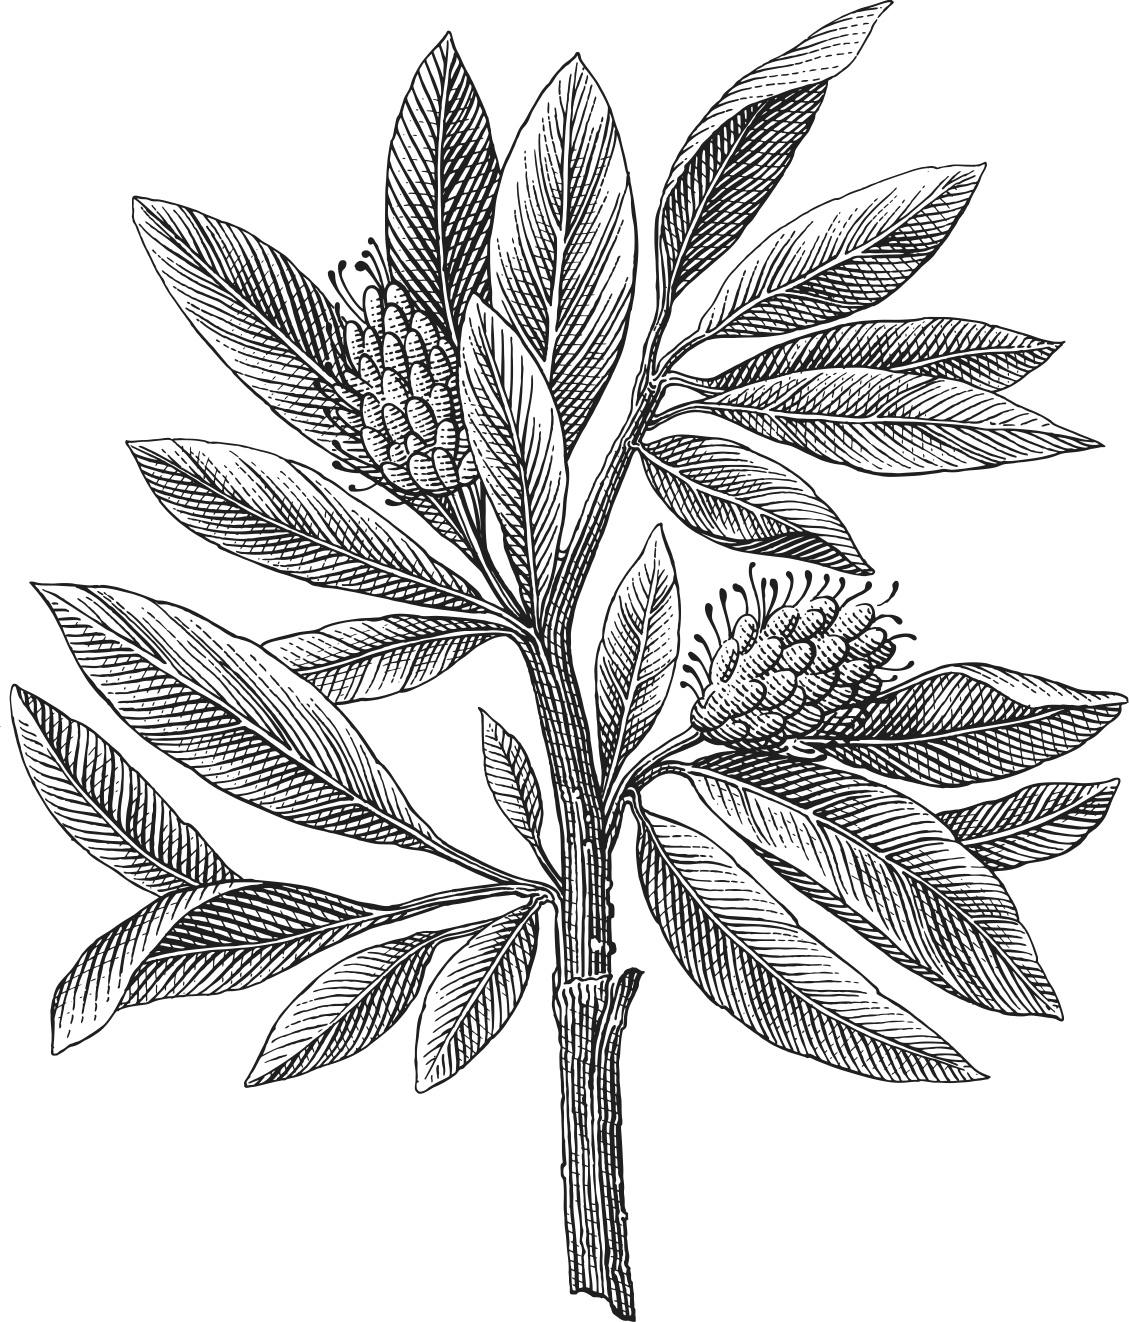
\includegraphics[keepaspectratio,scale=0.65]{lnu_etch.png} % Bakgrundsbild
    }
}
\newcommand\BackgroundPicLogo{
    \put(15,700){
    
\includegraphics[keepaspectratio,scale=0.10]{logo.png} % Logga i vänstra hörnet
    }
}

\newcommand{\horrule}[1]{\rule{\linewidth}{#1}} % Skapa hortisontell linje

\title{	\vspace{-10cm}
    \normalfont \normalsize
    \textsc{Linnaeus University} \\ [25pt] % Universitetes namn
    \horrule{0.5pt} \\[0.4cm] % Tunn linje högst upp
    \huge Laboration 4\\ % Arbetes titel
	\large \textcolor{gray}{1DV720 -- Server Administration}
    \horrule{0.5pt} \\[0.4cm] % Tunn linje längst ner
}

% \author{Jacob Lindehoff} % Författarnas namn

\date{\normalsize\today} % Dagens datum

\begin{document}
\AddToShipoutPicture*{\BackgroundPic} % Lägger in backgrundsbild på första sidan
\AddToShipoutPicture*{\BackgroundPicLogo}
\maketitle % Skriv ut titeln
\noindent % Tabba inte in på första meningen

%------------------------------------------------
%	Introduction
%------------------------------------------------
\section{Introduction}

For this module we will work with Active Directory and look at some of the concepts herein. After installing the A.D D.S role we start of by implementing an AGDLP strategy under certain parameters - the exact structure and naming convention will be up to you.

We will then setup group policies on these and assure that we have a proper delegation of control. 

%------------------------------------------------
%	Deadline
%------------------------------------------------
\section{Deadline}
There are two laboratory sessions connected to this module, at these sessions you are given the opportunity to get help if so needed. To be able to finish the modules you are likely needed to spend more time on your own.

\paragraph{Accounting} You will show your work and demonstrate your progress at any of these lab session, prepare a small document with an overview of your configuration/setup if needed for overview.


\pagebreak
%------------------------------------------------
%	Uppgift
%------------------------------------------------
\section{Assignment}
\begin{figure}[h]
\centering
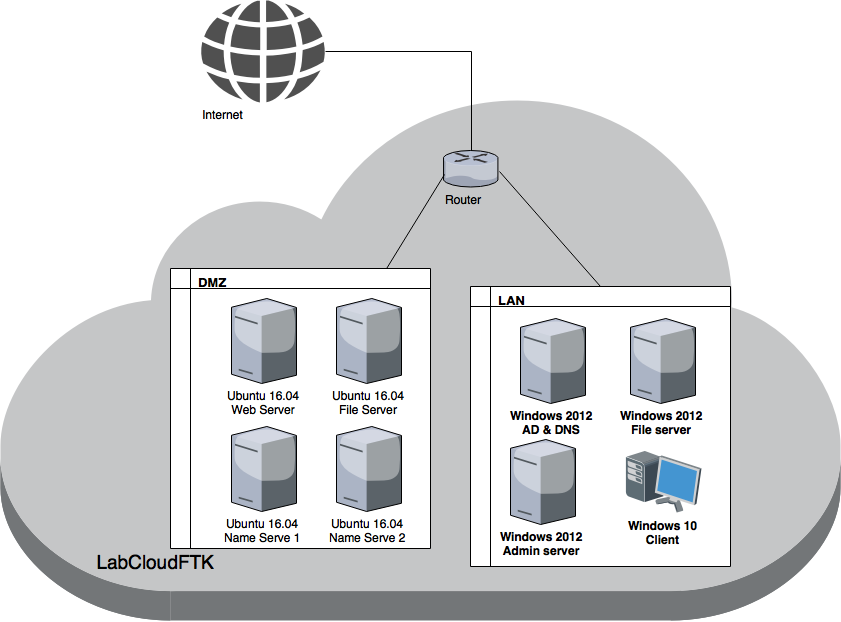
\includegraphics[width=1\linewidth]{./Lab04-Network}
\caption[Figure over network in Lab 4]{The network as it should be setup in Lab 4.}
\label{fig:network}
\end{figure}


The following fours sections with subtasks are the assignment:

\subsection{A.D DS Installation}
Add a new Windows Server 2012 Core and install the Active Directory Domain Services and promote the Windows server to a domain controller.

During the AD setup the server should configure a new DNS server. All the machines in the LAN should now be configured to use this DNS Server. Before you change all the network settings make sure that the DNS forwarder is correctly configure on the DNS server.

\subsection{A G/U DLP}
Adopt a AGDLP strategy for the environment specified in the Work Environment, add the users, and groups necessary to accomplish this. You then apply the AGDLP solution on your shares.

\subsection{Join Domain}
All internal clients and server in the LAN should join the A.D Domain. They should be visible under the computers tab in your A.D structure when you have joined.

\subsection{Delegation}
Make sure that the following delegations are in effect and make sure you use and AGDLP strategy for this too.
\paragraph{Human Resources:}
\begin{itemize}
	\item Should be able to read user information on all departments.
\end{itemize}

\paragraph{Call Center Manager:}
\begin{itemize}
	\item Should be able to add, modify and delete regular Callcenter users, but not managers.
	\item Should be able to add, modify and delete regular IT Support users.
\end{itemize}

\paragraph{IT Support:}
Not the same as administrators!
\begin{itemize}
	\item Should be able to add, modify, delete and reset password for Callcenter employees, but not Call Center managers.
	\item Should be able to add, modify and delete regular and reset password for Human resources users.
\end{itemize}

\subsection{Group Policies}
Apply group policies. Try at least 4 group policies and confirm that they are working and affecting only the users in the Call Center OU.
Apply a group policy that only affects the computers of your domain.
Confirm the policies are taking effect.

\subsection{Roaming profiles}
Create a roaming profile for at least one user.

\section{Requirements}
As in the previous labs, security is important and all machines should have there firewalls enabled. Firewall rules will be checked to be ‘decent’. Remember that if (as it should be) your firewall is properly setup you will need to make exception for the protocols you are implementing.
As previously your configuration should survive a reboot.

We will assume that the primary role of the company is a call center. We will also assume that we have a decent amount of employees ~50(but for the lab we don’t need to set up all of them!)
\subsection{Sections Layout}
In the environment there should exist the following departments, with employees:
\begin{itemize}
	\item IT Support
	\begin{itemize}
		\item Charles
	\end{itemize}
\end{itemize}
\begin{itemize}
	\item Human Resources
	\begin{itemize}
		\item Stina
		\item John
	\end{itemize}
\end{itemize}
\begin{itemize}
	\item Call Center
	\begin{itemize}
		\item Manager	
		\begin{itemize}
			\item Johan
		\end{itemize}
		
		\item Employees	
		\begin{itemize}
			\item Marcus
			\item Calina
		\end{itemize}
	\end{itemize}
\end{itemize}

\subsection{Resources}
The following resources should be shared according to your AGDLP solution:
\paragraph{Shares:}
\begin{itemize}
	\item Share:
	\begin{itemize}
		\item IT Support have full control
		\item Call Center Manager have read and modify Access
		\item  Call Center Employees have read access
		\item  Human resources have read access.
	\end{itemize}
	\item Managers:
	\begin{itemize}
		\item Call Center manager have full control
		\item  Call Center Employees have Read Access.
		\item  IT support have full control.
	\end{itemize}
\end{itemize}

\section{Work Enviroment}

You will be using FTK Lab Cloud to be able to accomplish this lab. You will find your credentials and tutorial on how to get started on this page: \href{https://coursepress.lnu.se/kurs/serveradministration/lab-cloud/}{https://coursepress.lnu.se/kurs/serveradministration/lab-cloud/}

Good luck!
\end{document}
